\section{Qualitätssicherung}
\label{sec:Qualitätssicherung}

\subsection{PDCA-Zyklus}
\label{sec:PDCA-Zyklus}

Quelle: der-prozessmanager.de \cite{pdcaZyklus}

Der PDCA-Zyklus (auch Deming-Kreis, Deming-Zyklus oder PDCA Kreislauf) bezeichnet ein grundlegendes Konzept im kontinuierlichen Verbesserungsprozess. Es dient der Weiterentwicklung von Produkten und Dienstleistungen sowie bei der Fehler-Ursache-Analyse. Der PDCA-Kreis besteht aus den vier sich wiederholenden Phasen: \hl{Plan-Do-Check-Act} (dt. Planen – Umsetzen – Überprüfen – Handeln). 

\begin{center}
	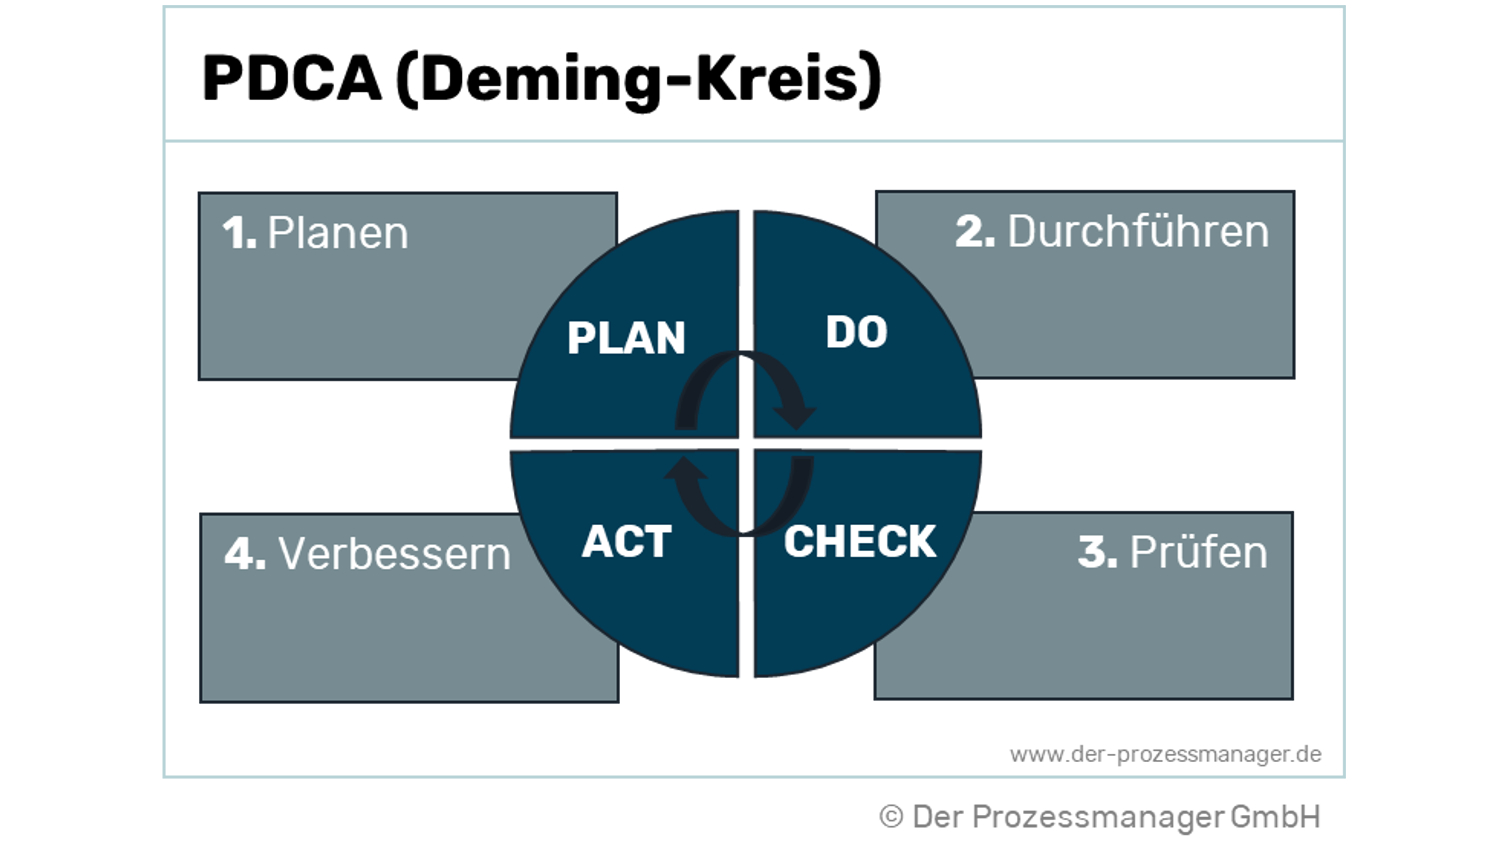
\includegraphics[scale=0.3]{Bilder/PDCA.png}
\end{center}

\textbf{Vorteile des PDCA-Kreises}

Der wesentliche Vorteil der PDCA-Methode ist wohl die \hl{einfache Anwendbarkeit}. Das Vorgehen hinsichtlich der spezifischen Aufgaben und Problemstellungen kann nahezu uneingeschränkt angepasst werden. Mit den Schritten Plan, Do, Check und Act bleibt dennoch ein solides Gerüst bestehen.

Weitere Vorteile:

\begin{itemize}
	\item Benötigt wenig Anleitung auf Grund des einfachen Aufbaus
	\item Die kreisförmige Konzeption ermöglicht ständige Verbesserung
	\item Durch den iterativen Ansatz lässt der PDCA-Zyklus Kontrolle und Analyse zu
\end{itemize}

\textbf{Nachteile des PDCA-Kreises}

Der große Vorteil des Demingkreises ist gleichzeitig auch ein wesentlicher Nachteil: \hl{Schnelle Problemlösungen lassen sich mit Hilfe des PDCA-Zyklus \mbox{\underline{nicht}} umsetzen}.

Nachteile auf einen Blick:

\begin{itemize}
	\item Unklare Definition der einzelnen Schritte kann zu falschem Einsatz führen
	\item Verbesserungen im Unternehmen müssen langfristig gedacht sein
	\item Eher ein reaktiver Ansatz, statt proaktiv
\end{itemize}

\subsection{Incident Management}
\label{sec:IncidentManagement}

Quelle: it-processmaps.com \cite{incidentManagement}

Incident Management verwaltet alle Incidents über ihren gesamten Lebenszyklus. Das primäre Ziel dieses ITIL-Prozesses besteht darin, einen IT Service für den Anwender so schnell wie möglich wieder herzustellen.

ITIL unterscheidet zwischen \hl{Incidents} (Service-Unterbrechungen) und \hl{Service Requests} (d. h. Anfragen von Anwendern, die keine Service-Unterbrechungen betreffen, wie z.B. das Zurücksetzen eines Passworts). Service-Unterbrechungen werden vom Incident-Management-Prozess behandelt, während Service-Anfragen vom \hl{Request Fulfilment} bearbeitet werden.

Der Incident-Management-Prozess kann auf verschiedenen Wegen angestoßen werden: Ein Anwender, Kunde oder Supplier kann eine Störung melden, technisches Personal kann einen (drohenden oder tatsächlichen) Ausfall feststellen, oder ein Incident kann automatisch von einem Event-Monitoring-System ausgelöst werden.

Alle \hl{Incidents sollten in Incident Records festgehalten werden}, so dass ihr Status verfolgt und ihr vollständiger Verlauf dokumentiert werden kann. Die initiale Kategorisierung und Priorisierung der Incidents ist ein wichtiger Schritt zur Bestimmung, wie mit dem Incident verfahren wird und wieviel Zeit für dessen Lösung verfügbar ist.

Falls möglich, sollten Incidents mit anderen Incidents, Problems und Known Errors verknüpft werden.

\subsection{Service Level Agreement (SLA), Servicelevel 1-3}
\label{sec:ServiceLevelAgreement}

Quelle: Amazon \cite{SLAAmazon}

Ein Service Level Agreement (SLA) ist ein Vertrag mit einem Outsourcing- und Technologieanbieter, in dem das \hl{Serviceniveau} festgelegt ist, das ein Anbieter dem Kunden zu liefern verspricht. Sie gibt \hl{Aufschluss über Kennzahlen wie Betriebszeit, Lieferzeit, Reaktionszeit und Lösungszeit}. In einem SLA ist auch festgelegt, was zu tun ist, wenn die Anforderungen nicht erfüllt werden, z. B. zusätzliche Unterstützung oder Preisnachlässe. SLAs werden in der Regel zwischen einem Kunden und einem Service-Anbieter vereinbart, obwohl auch Geschäftseinheiten innerhalb desselben Unternehmens untereinander SLAs abschließen können.

\subsection{Testen}
\label{sec:Testen}

\subsubsection{Klassifizierung von Testverfahren}
\label{sec:KlassifizierungTestverfahren}

\begin{itemize}
	\item Wer testet?
	\begin{itemize}
		\item Mensch (manuell) vs. Maschine (automatisch)
		\item Entwickler vs. Benutzer
	\end{itemize}
	\item Was wird getestet?
	\begin{itemize}
		\item Komponente (Unit-Test/Funktionstest/Klassentest) vs. Integration vs. System (End-to-End)
		\item Testpyramide
	\end{itemize}
	\item Wie wird getestet?
	\begin{itemize}
		\item Bottom-Up vs. Top-Down
		\item statisch (Kompilierzeit) vs. dynamisch (Laufzeit)
		\item ohne Kenntnis des Codes (Blackbox) vs. mit Kenntnis des Codes (Whitebox)
		\item explorativ
		\item Schreibtischtest/Review
	\end{itemize}
	\item Wann wird getestet?
	\begin{itemize}
		\item Vor vs. nach der Entwicklung
		\item Abnahmetest
	\end{itemize}
	\item Warum wird getestet?
	\begin{itemize}
		\item Regressionstest
		\item Lasttest/Belastungstest
		\item Smoketest
	\end{itemize}
\end{itemize}



\subsection{Versionsverwaltung}
\label{sec:Versionsverwaltung} 


